\subsection{Automaten}

\begin{figure}[h]
  \centering
  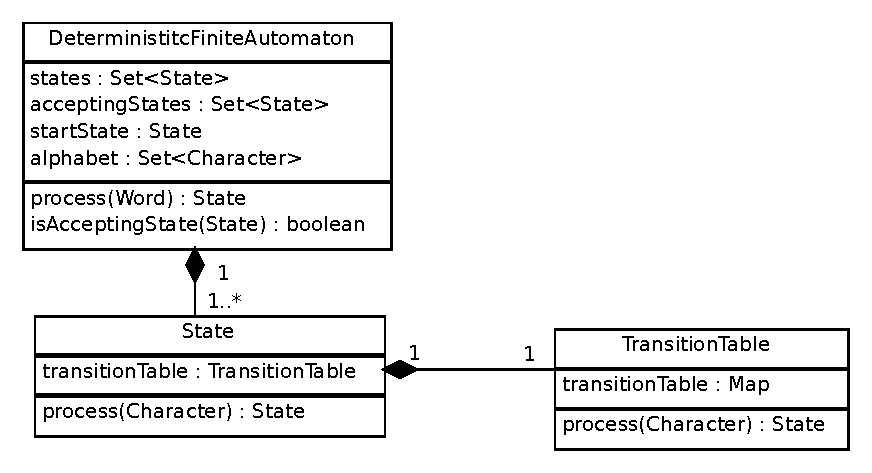
\includegraphics[width=0.5\textwidth]{images/dfa_classdiag_simple.pdf}
  \caption[DFA Klassendiagramm vereinfacht]{DFA Klassendiagramm vereinfacht}
  \label{fig:dfa_classdiag_simple}
\end{figure}


Das Quintupel Modell ($Q$, $\Sigma$, $\delta$, $q0$, $F$) wurde wie folgt implementiert:

\begin{tabular}{ l | l }
  \hline
  $Q$ & Die Menge der Zustände wurde als Set von States implementiert.  \\
  \hline
  $\Sigma$ & 5 \\
  \hline
  $\delta$ & 8 \\
  \hline
  $\q0$ & 8 \\
  \hline
  $F$ & 8 \\
  \hline 
\end{tabular}

